%%%%%%%%%%%%%%%%%%%%%%%%%%%%%%%%%%%%%%
% LaTeX poster template
% Created by Nathaniel Johnston
% August 2009
% http://www.nathanieljohnston.com/index.php/2009/08/latex-poster-template/
%%%%%%%%%%%%%%%%%%%%%%%%%%%%%%%%%%%%%%

\documentclass[final]{beamer}
%\usepackage[scale=1.24]{beamerposter}
  \usepackage[orientation=portrait,size=a0,scale=1.7,debug]{beamerposter}                       % e.g. for DIN-A0 poster
\usepackage{etex}
\reserveinserts{28}
\usepackage{graphicx}			% allows us to import images
%\usepackage{caption} % For empty captions
\usepackage{caption}
\usepackage{subcaption}
%-----------------------------------------------------------
% Define the column width and poster size
% To set effective sepwid, onecolwid and twocolwid values, first choose how many columns you want and how much separation you want between columns
% The separation I chose is 0.024 and I want 4 columns
% Then set onecolwid to be (1-(4+1)*0.024)/4 = 0.22
% Set twocolwid to be 2*onecolwid + sepwid = 0.464
%-----------------------------------------------------------

\newlength{\sepwid}
\newlength{\onecolwid}
\newlength{\twocolwid}
\newlength{\threecolwid}
%\newlength{\ppaperwidth}
%\newlength{\ppaperheight}
%\setlength{\ppaperwidth}{48in}
%\setlength{\ppaperheight}{36in}
\setlength{\sepwid}{0.024\paperwidth}
\setlength{\onecolwid}{0.45\paperwidth}
\setlength{\twocolwid}{0.63\paperwidth}
\setlength{\threecolwid}{0.95\paperwidth}
\setlength{\topmargin}{-0.5in}
\usetheme{confposter}

\newcommand{\vsp}{\vspace*{2cm}}


%-----------------------------------------------------------
% Define colours (see beamerthemeconfposter.sty to change these colour definitions)
%-----------------------------------------------------------

\setbeamercolor{block title}{fg=dblue,bg=white}
\setbeamercolor{block body}{fg=black,bg=white}
\setbeamercolor{block alerted title}{fg=white,bg=dblue!80}
\setbeamercolor{block alerted body}{fg=black,bg=dblue!10}


\usepackage{times}
\usepackage{helvet}
%\usepackage{bookman}
\usepackage{palatino}


%multi column itemize
\usepackage{etoolbox}
\usepackage{multicol}

\usepackage{graphicx}
\usepackage{amssymb,amsmath}

\usepackage{times}
\usepackage{latexsym}
\usepackage{color}

\usepackage{url}


\definecolor{gray}{rgb}{0.5,0.5,0.5}
\definecolor{ForestGreen}{HTML}{228B22}


%%%%%%%%%%%%%%%%%%%%%%%%%%%%%%%%%%%%%%%%%%%%%%%%%%%%%%%%%%%%%%%%%%%%%%%%%%%%%%%%
% Multicol Settings
%%%%%%%%%%%%%%%%%%%%%%%%%%%%%%%%%%%%%%%%%%%%%%%%%%%%%%%%%%%%%%%%%%%%%%%%%%%%%%%%
\setlength{\columnsep}{0.7em}
\setlength{\columnseprule}{0mm}


%%%%%%%%%%%%%%%%%%%%%%%%%%%%%%%%%%%%%%%%%%%%%%%%%%%%%%%%%%%%%%%%%%%%%%%%%%%%%%%%
% Save space in lists. Use this after the opening of the list
%%%%%%%%%%%%%%%%%%%%%%%%%%%%%%%%%%%%%%%%%%%%%%%%%%%%%%%%%%%%%%%%%%%%%%%%%%%%%%%%
\newcommand{\compresslist}{%
\setlength{\itemsep}{1.2pt}%
\setlength{\parskip}{0pt}%
\setlength{\parsep}{0pt}%
}




\newcommand{\uur}[1]{\textcolor{red}{#1}}
\newcommand{\uuxr}[1]{\textcolor{red}{#1}}
\newcommand{\uuxo}[1]{\textcolor{uuxorange}{#1}}
%\newcommand{\uuxo}[1]{\emph{#1}}
%\newcommand{\uuxb}[1]{\textcolor{uuxb}{#1}}
\newcommand{\uuxb}[1]{\textcolor{uuxblue}{#1}}
%\newcommand{\uudb}[1]{\textcolor{uu2darkblue}{#1}}
%\newcommand{\uut}[1]{\textcolor{uu2terra}{#1}}
%\newcommand{\uurho}[1]{\textcolor{uu2rhodamine}{#1}}
%\newcommand{\uuxg}[1]{\textcolor{uuxgreen}{#1}}

\newcommand{\uuxg}[1]{\textcolor{ForestGreen}{#1}}


%\newcommand{\uuxo}[1]{\textcolor{uuxorange}{#1}}







%%UU colors:

%	naam 	pms 	cmyk (%) uncoated 	rgb 	html
%% Corporate colors
%	UU geel 	110 U 	0-11,5-94-15 	219-189-0 	#dbbd00
\definecolor{uuyellow}{cmyk}{0,0.115,0.94,0.15}
%	uu rood 	186 U 	7-93-71-1 	215-0-68 	#d70044
\definecolor{uured}{cmyk}{0,0.91,0.76,0.06}
%	zwart 	  	  	  	#000000

%% Extra corporate colors
%	oranje 	143 	0-30-90-0 	243-185-39 	#f3b927
\definecolor{uuxorange}{cmyk}{0,0.3,0.9,0}
%	rood 	704 	20-100-90-10 	146-19-40 	#921328
\definecolor{uuxred}{cmyk}{0.2,1,0.9,0.1}
%	groen 	340 	90-15-70-0 	0-140-107 	#008c6b
\definecolor{uuxgreen}{cmyk}{0.9,0.15,0.7,0}
%	blauw 	293 	90-55-0-0 	58-102-174 	#3a66ae
\definecolor{uuxblue}{cmyk}{0.9,0.55,0.0,0.0}
%	paars 	259 	70-100-20-5 	106-18-105 	#6a1269
\definecolor{uuxpurple}{cmyk}{0.7,1,0.2,0.05}

%% Secondary palette
%	donkerrood 	202 	30-100-90-30 	105-3-29 	#69031d
\definecolor{uu2darkred}{cmyk}{0.3,1,0.9,0.3}
%	terra 	1525 	15-50-100-0 	199-126-30 	#c77e1e
\definecolor{uu2terra}{cmyk}{0.15,0.5,1,0}
%	lichtgeel 	604 	0-5-100-0 	248-235-0 	#f8eb00
\definecolor{uu2lightyellow}{cmyk}{0,0.05,1,0}
%	donkergroen 	342 	100-30-80-20 	0-75-51 	#004b33
\definecolor{uu2darkgreen}{cmyk}{1,0.3,0.8,0.2}
%	olijfgroen 	397 	20-5-100-0 	176-198-0 	#b0c600
\definecolor{uu2olive}{cmyk}{0.2,0.05,1,0}
%	lichtgroen 	381 	10-0-100-0 	215-230-0 	#d7e600
\definecolor{uu2lightgreen}{cmyk}{0.1,0,1,0}
%	donkerblauw 	2748 	100-90-20-10 	50-36-98 	#322462
\definecolor{uu2darkblue}{cmyk}{1,0.9,0.2,0.1}
%	azuurblauw 	313 	100-25-20-0 	0-131-166 	#0083a6
\definecolor{uu2azure}{cmyk}{1,0.25,0.2,0}
%	lichtblauw 	305 	60-0-10-0 	111-197-226 	#6fc5e2
\definecolor{uu2lightblue}{cmyk}{0.6,0,0.1,0}
%	donkerpaars 	511 	70-90-50-30 	59-27-50 	#3b1b32
\definecolor{uu2darkpurple}{cmyk}{0.7,0.9,0.5,0.3}
%	fuchsia 	234 	30-100-40-5 	142-6-78 	#8e064e
\definecolor{uu2fuchsia}{cmyk}{0.3,1,0.4,0.05}
%	fuchsia 	Rhodamine red 	6-100-10-0 	199-0-110 	#c7006e
\definecolor{uu2rhodamine}{cmyk}{0.06,1,0.1,0}

\title{\Large{Functional Programming Laboratory}}

\author{School of Computer Science}
%\institute{$\;$}
\institute{University of Nottingham}

\begin{document}
%
%
%
\begin{frame}[t]\vspace{-2cm}
\begin{columns}[t]

%    \begin{column}{\sepwid}\end{column}			% empty spacer column


\begin{column}{\threecolwid}

	\begin{center}
	The aim of the Functional Programming Lab is to develop \uuxg{simple but powerful techniques} for \textcolor{uuxblue}{writing} and \textcolor{uuxblue}{reasoning about programs}, by recognising and exploiting their \textcolor{uuxblue}{underlying mathematical structure}. Most of our work takes place within the context of \textcolor{uuxblue}{functional languages} such as \textcolor{uuxblue}{Haskell} and \textcolor{uuxblue}{Agda}, which are at the forefront of \uuxg{programming language research}, and provide ideal vehicles for research of this nature. 
%	\\[1.0cm]
%\vspace{1cm}
%See also \url{http://fp.cs.nott.ac.uk/} for the \textcolor{uuxblue}{group website}.
\end{center}

 \begin{column}{\sepwid}\end{column}			% empty spacer column

\end{column}
\end{columns}

\begin{columns}[t]
    \begin{column}{\sepwid}\end{column}			% empty spacer column


\begin{column}{\onecolwid}


\begin{block}{Undergraduate research projects}
Various topics: \\[0.3cm]
\begin{itemize}
	\item \textbf{General Haskell} 
	\item \textbf{Implementing video games}
	\item \textbf{Theorem proving} 
	\item \textbf{Compilers and interpreters} 
	\item \textbf{Foundations of programming}
	\item \textbf{Type theory}
\end{itemize}
\end{block}


\vsp
\begin{figure}%
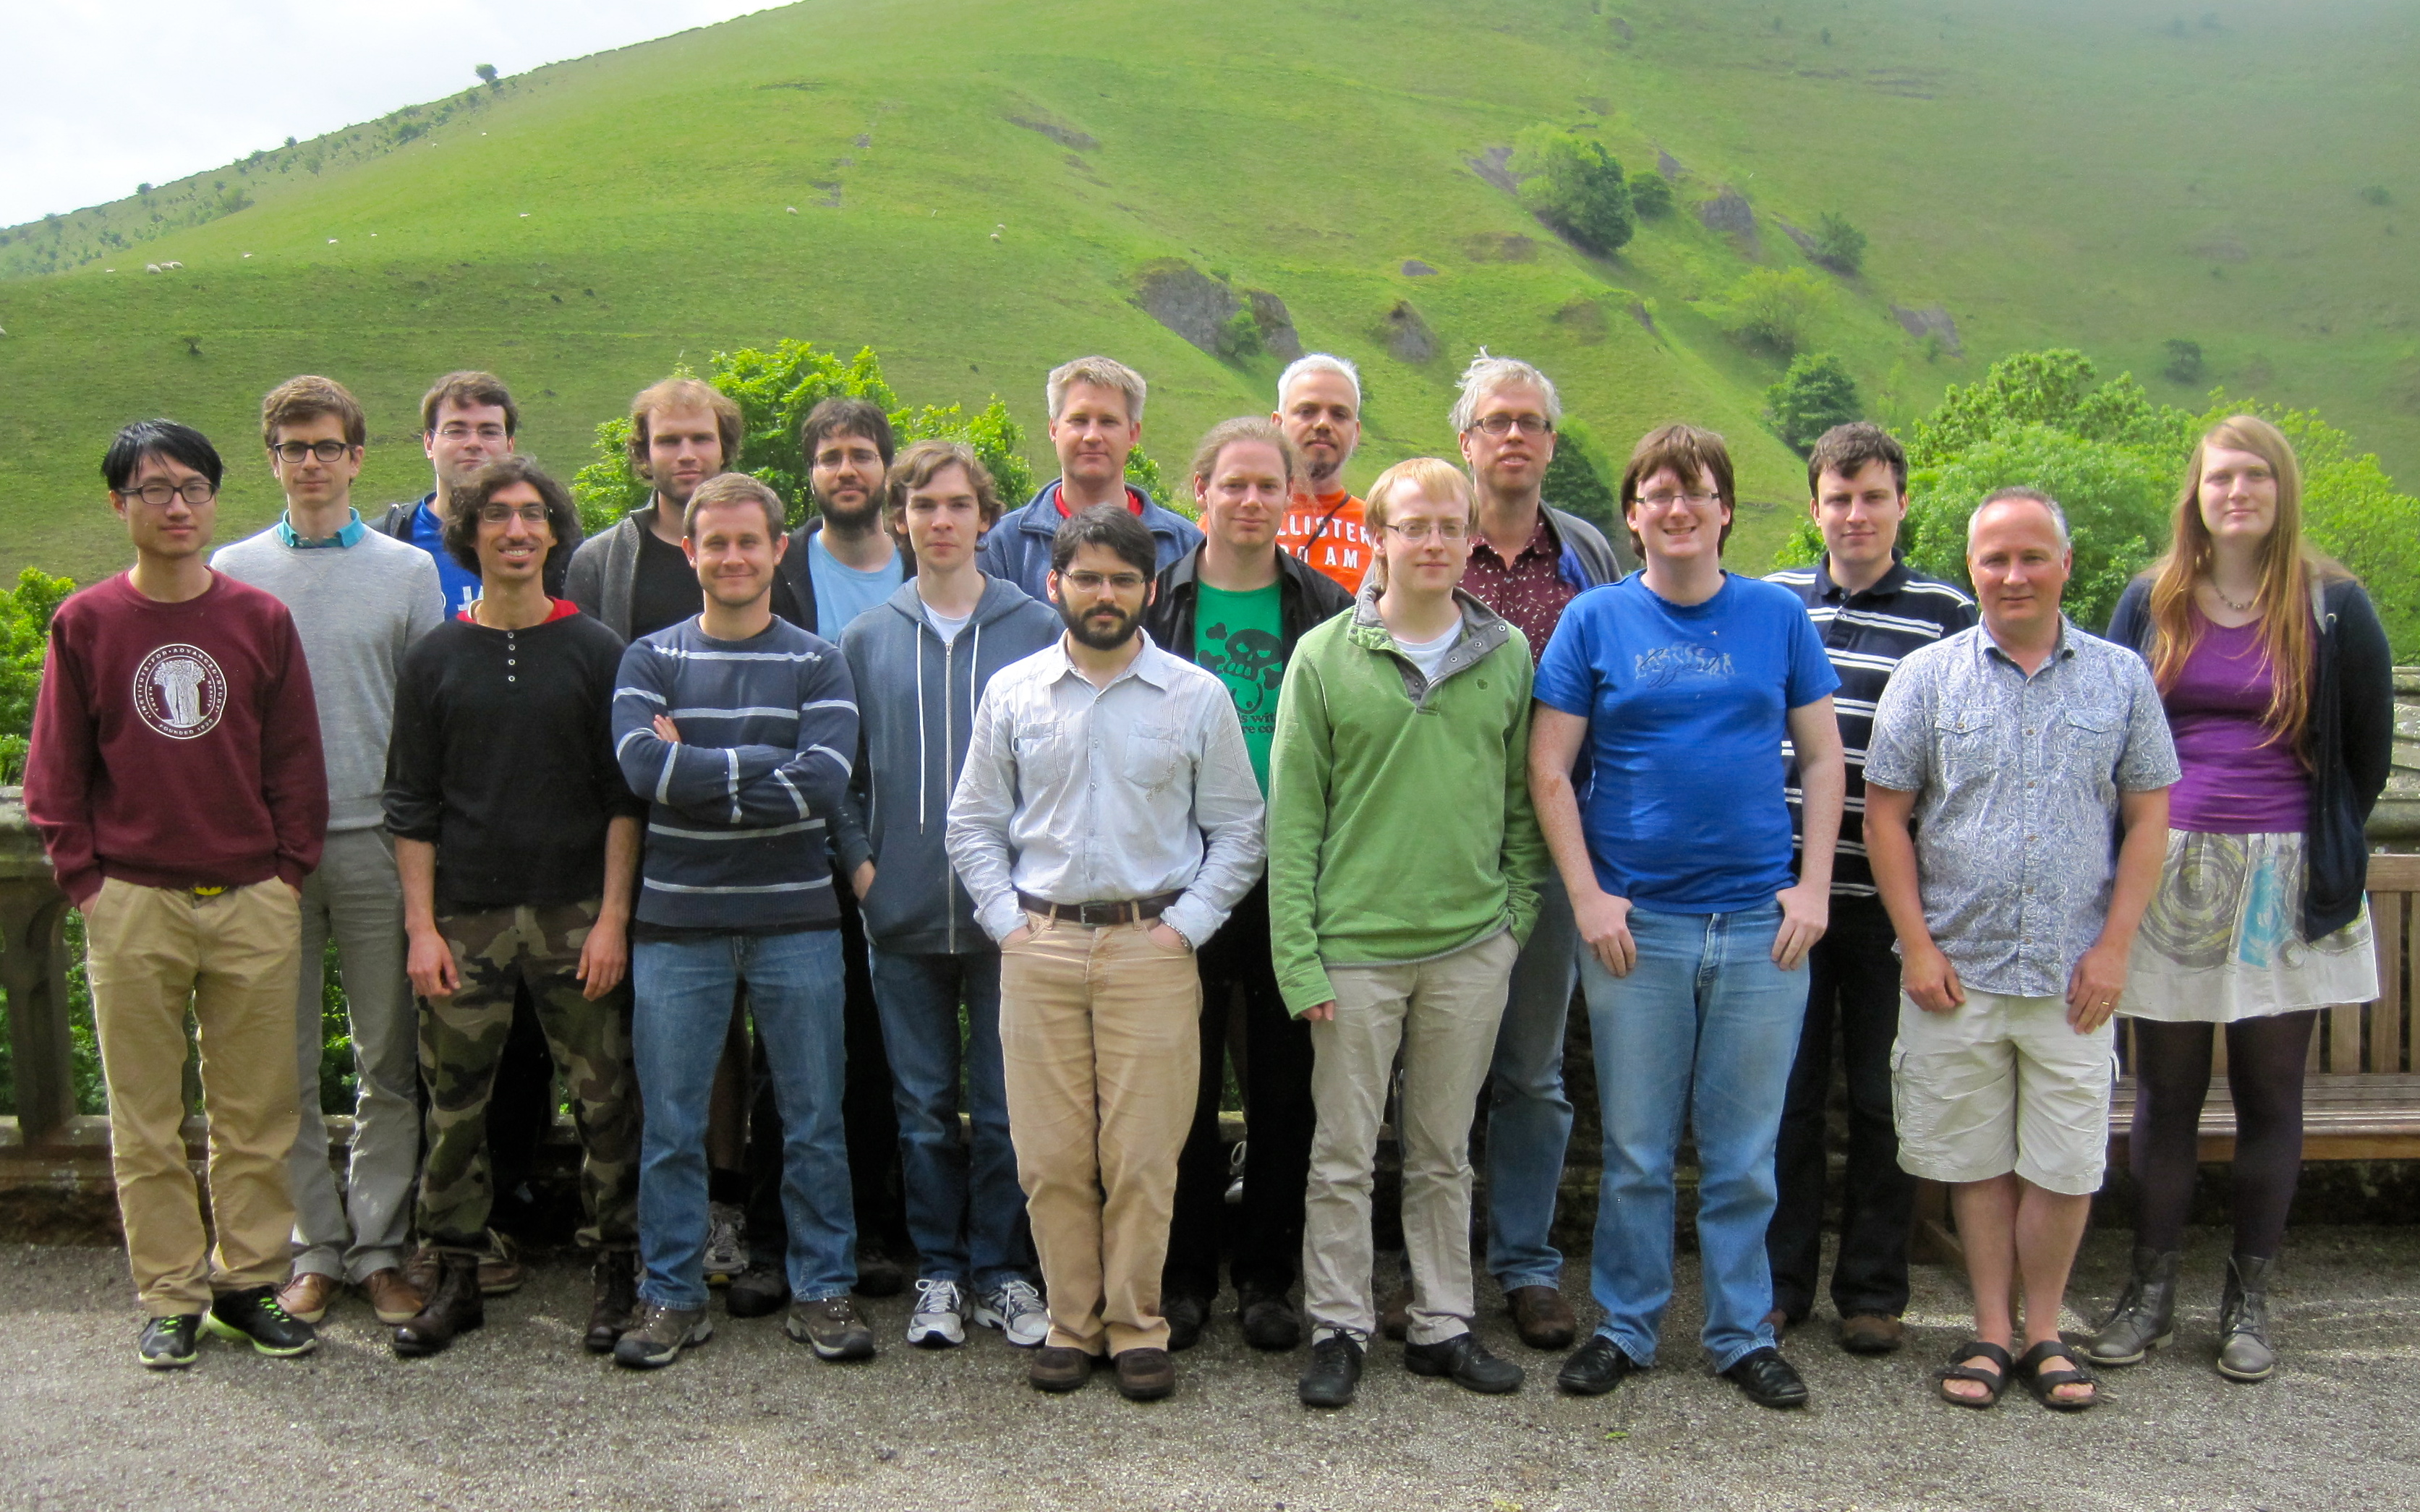
\includegraphics[width=\onecolwid]{FP-LAB-2013.jpg}%
%\caption{The current members of the FP lab}%
%\label{}%
\end{figure}
\begin{center}\vspace{-0.5cm}
	The current members of the FP lab. 
\end{center}
\vsp

%\begin{block}{Example research project}
%Insert example from last year?

%\begin{center}
%	Some figure:
%\end{center}
%\begin{figure}%
%%\includegraphics[width=\columnwidth]{filename}%
%%\caption{}%
%%\label{}%
%\end{figure}
%\end{block}



\end{column}













\begin{column}{\sepwid}\end{column}			% empty spacer column


\begin{column}{\onecolwid}

%\vsp

\begin{block}{Research in the FP lab}
%Our research spans a range of topics in the area of \uuxb{functional programming} including:
Our research spans a \uuxb{range of topics} including:
%
%
\begin{itemize}\vspace{-.5cm}
\begin{multicols}{2}
{
	\item Category theory
	\item Corecursive structures
	\item Compiler correctness
	\item Declarative debugging
	\item Hybrid modelling
	\item Reactive programming
	\item Mathematical logic
	\item Program optimisation
	\item Proof assistants
	\item Quantum computing
	\item Type theory
	\item Homotopy type theory
}
\end{multicols}	
\end{itemize}
\end{block}

\vsp


\begin{figure}%

\includegraphics[width=\onecolwid]{haskell-logo-with-name.jpg}
\end{figure}

\end{column}

\begin{column}{\sepwid}\end{column}			% empty spacer column


\end{columns}
\begin{columns}[t]

\begin{column}{\threecolwid}

\begin{block}{Internships in the FP lab}
\begin{center}	
We're also interested in students to do \textcolor{uuxblue}{summer internships}!
\end{center}
\end{block}

\vsp

\begin{block}{Research staff}


\begin{figure}
        \centering
        \begin{subfigure}[b]{0.2\textwidth}
                \centering
                
\includegraphics[height=12cm]{thorstenaltenkirch.jpg}
                \caption*{Thorsten Altenkirch}
        \end{subfigure}%
        ~ %add desired spacing between images, e. g. ~, \quad, \qquad etc.
          %(or a blank line to force the subfigure onto a new line)
        \begin{subfigure}[b]{0.2\textwidth}
                \centering
                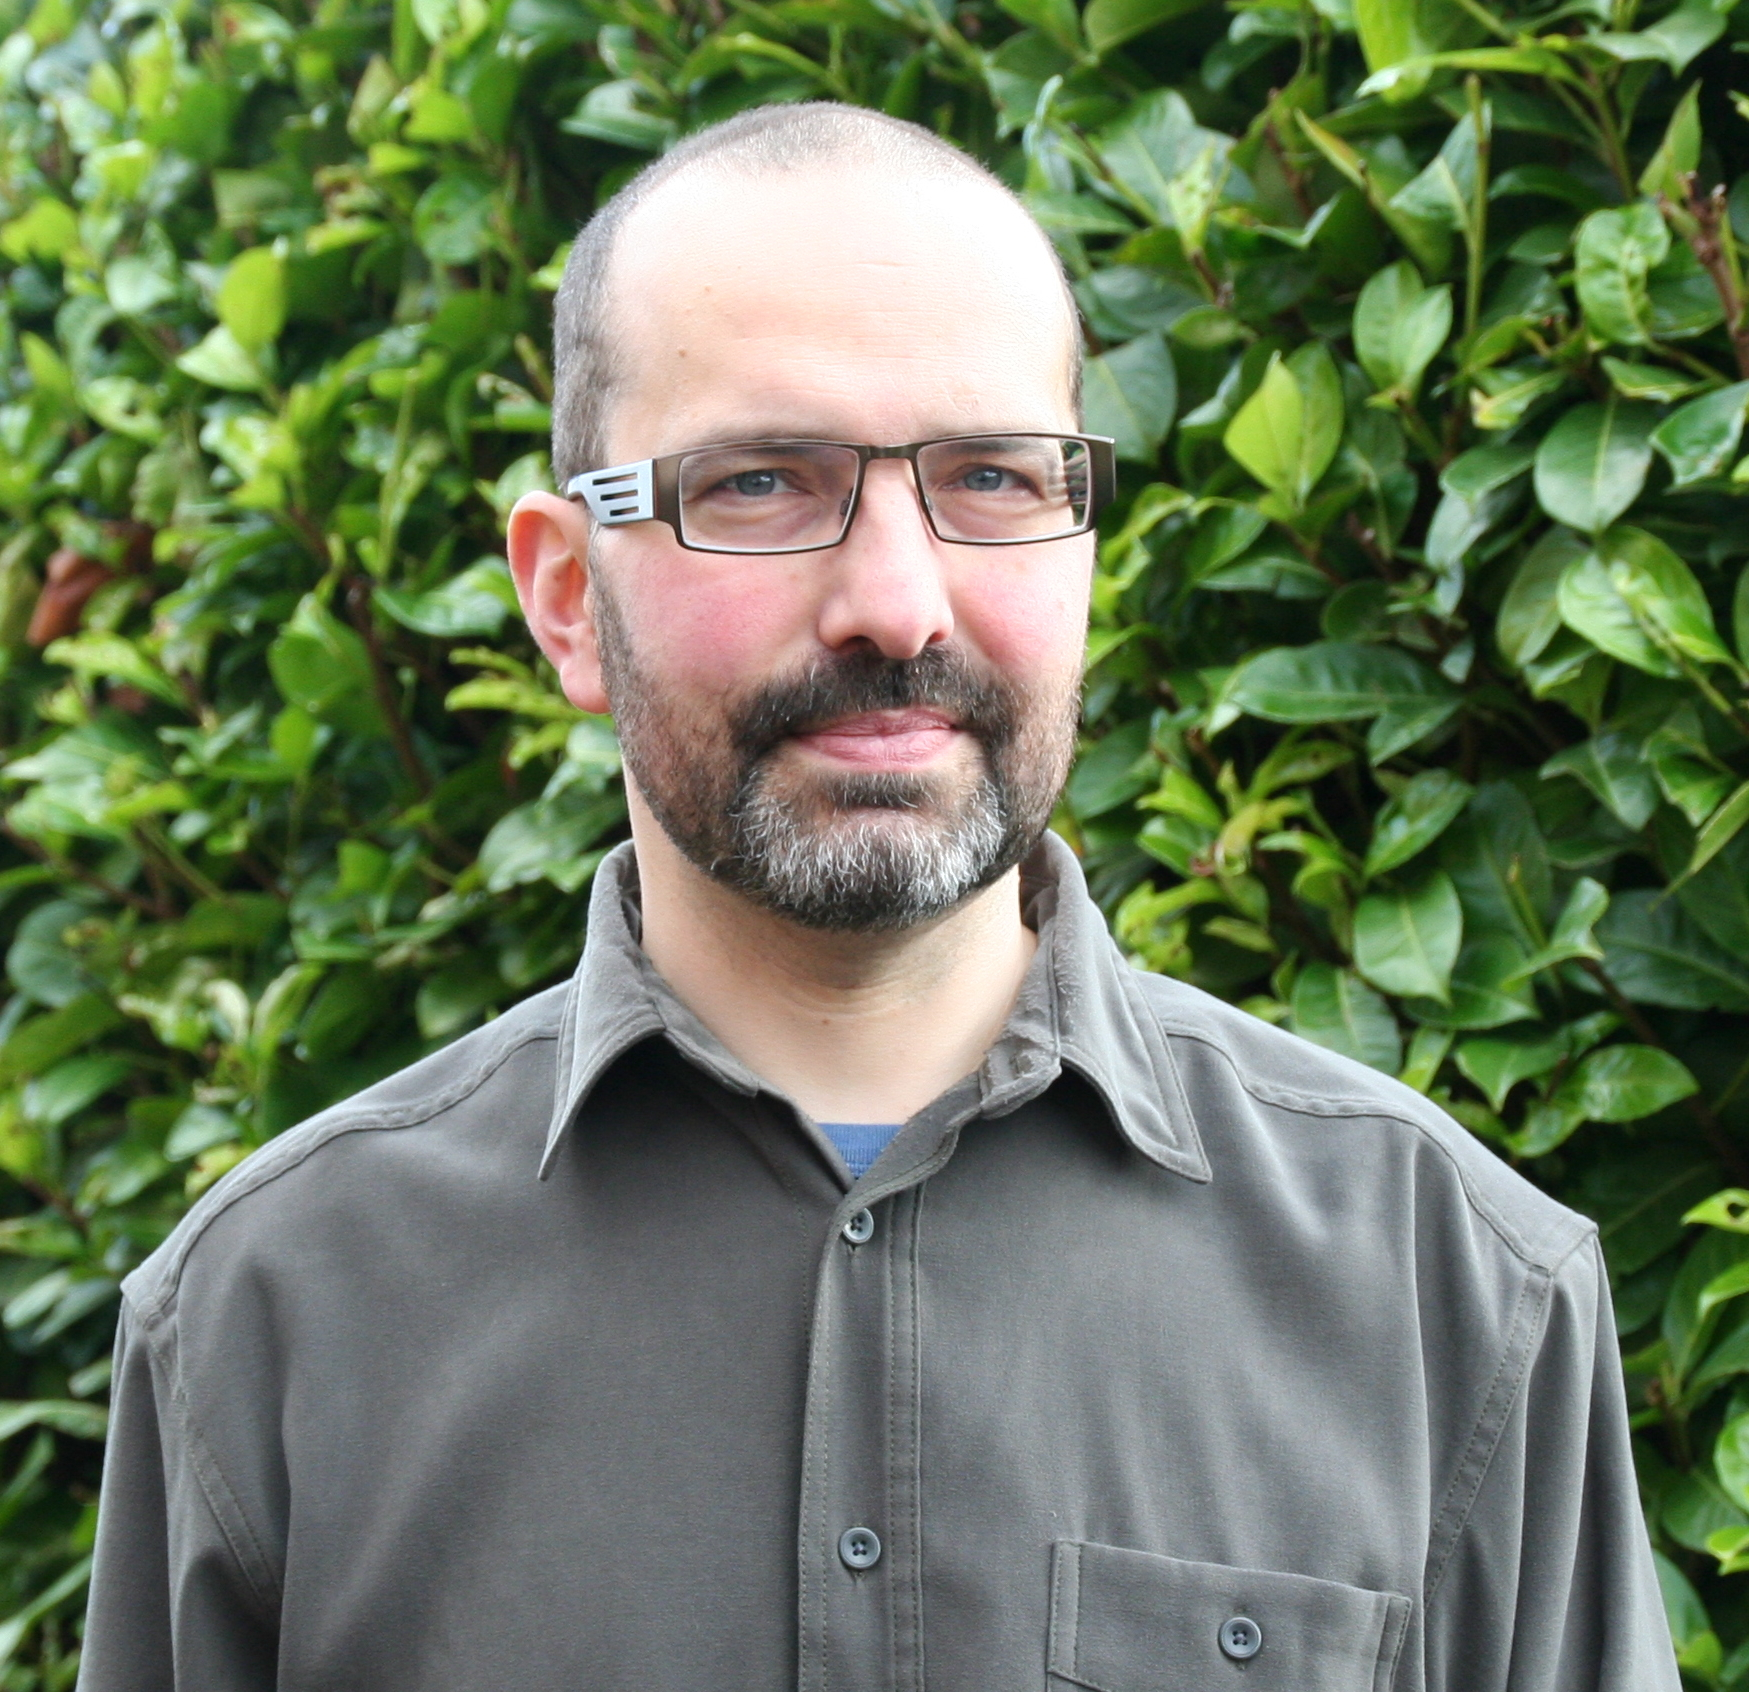
\includegraphics[height=12cm]{venanzio_capretta_portrait.jpg}
                \caption*{Venanzio Capretta}
        \end{subfigure}
        ~ %add desired spacing between images, e. g. ~, \quad, \qquad etc.
          %(or a blank line to force the subfigure onto a new line)
        \begin{subfigure}[b]{0.2\textwidth}
                \centering
                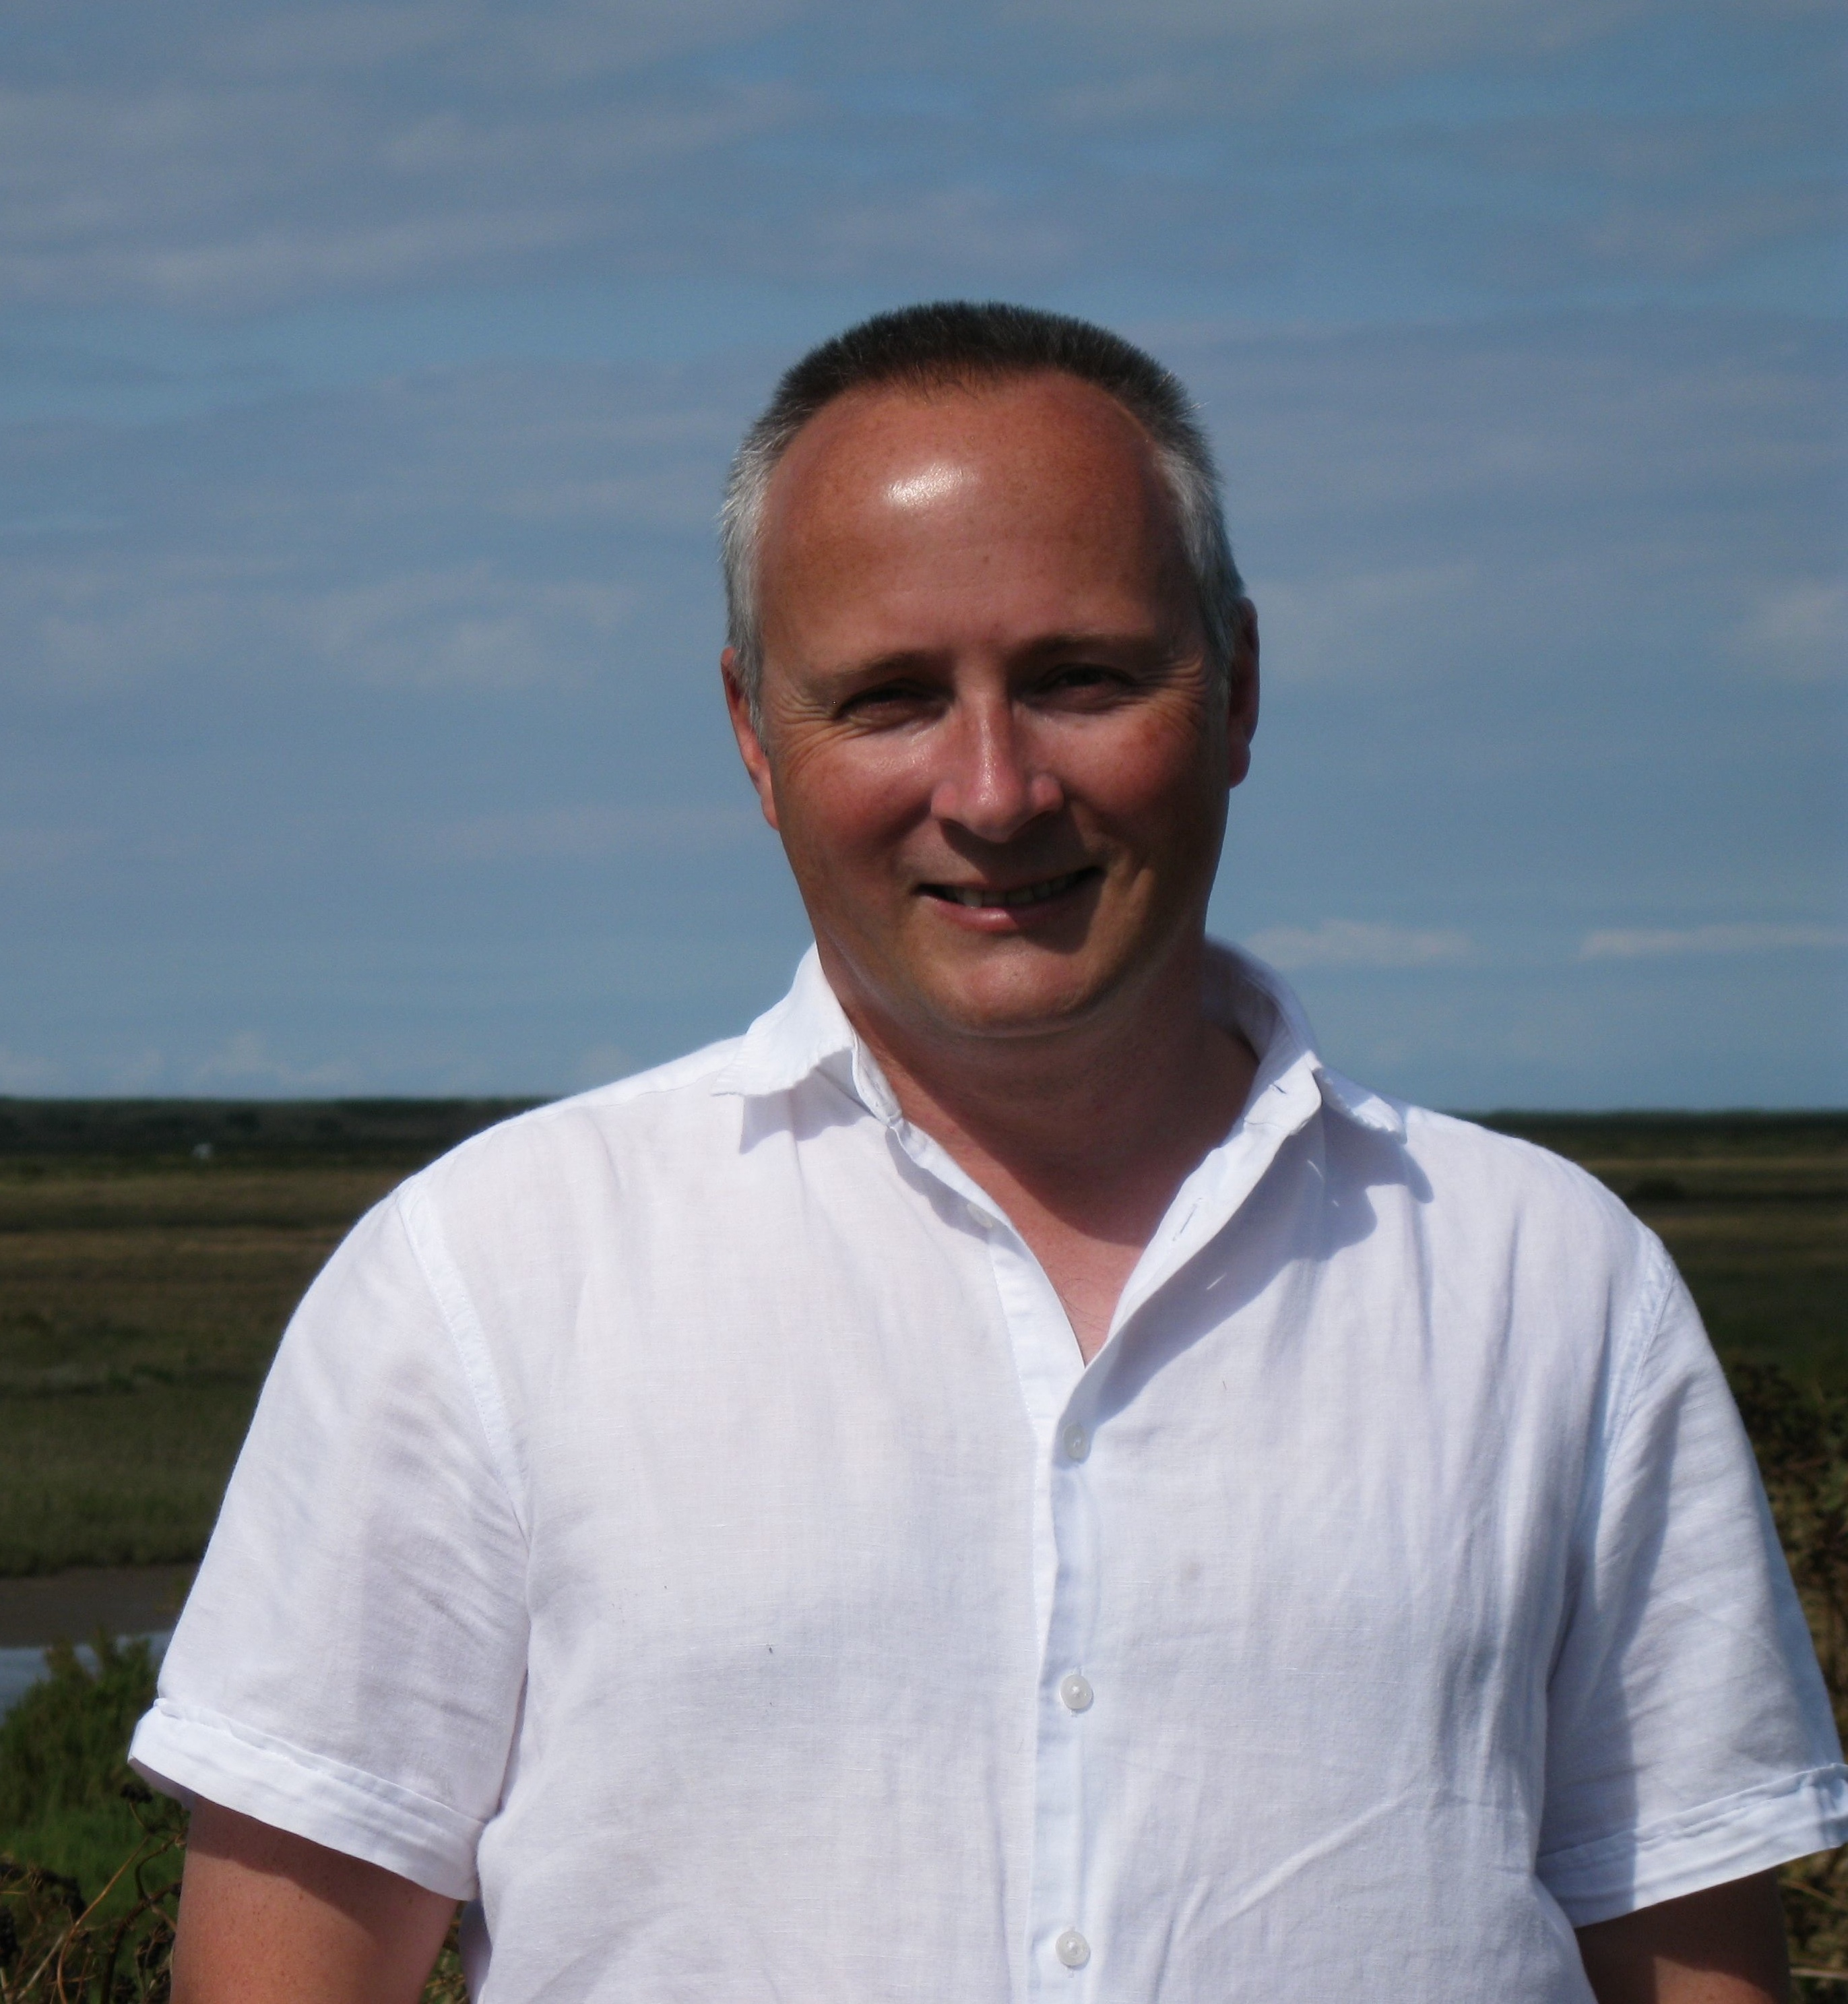
\includegraphics[height=12cm]{hutton2.jpg}
                \caption*{Graham Hutton}
        \end{subfigure}
        \begin{subfigure}[b]{0.2\textwidth}
                \centering
                
\includegraphics[height=12cm]{henriknilsson.jpg}
                \caption*{Henrik Nilsson}
        \end{subfigure}
\end{figure}
\end{block}

\end{column}

\end{columns}


\end{frame}

\end{document}







